%%%%%%%%%%%%%%%%%%%%%%%%%%%%%%%%%%%%%%%%%
% fphw Assignment
% LaTeX Template
% Version 1.0 (27/04/2019)
%
% This template originates from:
% https://www.LaTeXTemplates.com
%
% Authors:
% Class by Felipe Portales-Oliva (f.portales.oliva@gmail.com) with template 
% content and modifications by Vel (vel@LaTeXTemplates.com)
%
% Template (this file) License:
% CC BY-NC-SA 3.0 (http://creativecommons.org/licenses/by-nc-sa/3.0/)
%
%%%%%%%%%%%%%%%%%%%%%%%%%%%%%%%%%%%%%%%%%

%----------------------------------------------------------------------------------------
%	PACKAGES AND OTHER DOCUMENT CONFIGURATIONS
%----------------------------------------------------------------------------------------

\documentclass[
	12pt, % Default font size, values between 10pt-12pt are allowed
	%letterpaper, % Uncomment for US letter paper size
	%spanish, % Uncomment for Spanish
]{fphw}

% Template-specific packages
\usepackage[utf8]{inputenc} % Required for inputting international characters
\usepackage[T1]{fontenc} % Output font encoding for international characters
\usepackage{mathpazo} % Use the Palatino font

\usepackage{graphicx} % Required for including images

\usepackage{booktabs} % Required for better horizontal rules in tables

\usepackage{listings} % Required for insertion of code
\usepackage[colorlinks,linkcolor=red]{hyperref}
\usepackage{enumerate} % To modify the enumerate environment
%codes setting
\RequirePackage{listings}
\RequirePackage{xcolor}
\definecolor{dkgreen}{rgb}{0,0.6,0}
\definecolor{gray}{rgb}{0.5,0.5,0.5}
\definecolor{mauve}{rgb}{0.58,0,0.82}
\lstset{
	numbers=left,  
	frame=tb,
	aboveskip=3mm,
	belowskip=3mm,
	showstringspaces=false,
	columns=flexible,
	framerule=1pt,
	rulecolor=\color{gray!35},
	backgroundcolor=\color{gray!5},
	basicstyle={\ttfamily},
	numberstyle=\tiny\color{gray},
	keywordstyle=\color{blue},
	commentstyle=\color{dkgreen},
	stringstyle=\color{mauve},
	breaklines=true,
	breakatwhitespace=true,
	tabsize=3,
}
%----------------------------------------------------------------------------------------
%	ASSIGNMENT INFORMATION
%----------------------------------------------------------------------------------------

\title{Homework \#2} % Assignment title

\author{Hang Chen} % Student name

\date{September 22, 2020}

\institute{Boise State University \\ Department of geoscience} % Institute or school name

\class{GEOS 422 / GEOPH 522: Data Analysis and Geostatistics} % Course or class name


%----------------------------------------------------------------------------------------

\begin{document}

\maketitle % Output the assignment title, created automatically using the information in the custom commands above

%----------------------------------------------------------------------------------------
%	ASSIGNMENT CONTENT
%----------------------------------------------------------------------------------------

\section*{Question 1}

\begin{problem}
	Assuming no uncertainty and large enough sample size, we will use the complete dataset to define the true statistics of the underlying distribution of elevation. Calculate the "true" 	minimum $q_0$, maximum $q_{100}$, standard deviation $\sigma$ and mean $\mu$, using the entire dataset.
\end{problem}




%------------------------------------------------

\subsection*{Answer}

The minimum, maximum, mean and standard deviation of each dataset is calculated by the codes:
\begin{lstlisting}[language=Matlab,escapeinside=``]
q0=nanmin(D) %calculate the minimum and print it in command window
q100=nanmax(D) % calcualate the maximum and print it in command window
mu=nanmean(D) % calcualate the mean and print it in command window
sigma=nanstd(D) % calcualate the standard deviation and print it in command window
\end{lstlisting}

The results show that the 	minimum $q_0$ of dataset is  2.7356e+03, the  maximum $q_{100}$ of dataset is   2.9198e+03,mean $\mu$ equals to 2.7948e+03 and standard deviation $\sigma$ equals to  40.1700.




%----------------------------------------------------------------------------------------

\section*{Question 2}

\begin{problem}
Plot a relative density histogram of the entire elevation dataset
	
\end{problem}

%------------------------------------------------

\subsection*{Answer}

The result is

\begin{figure}[htbp]
	\centering
	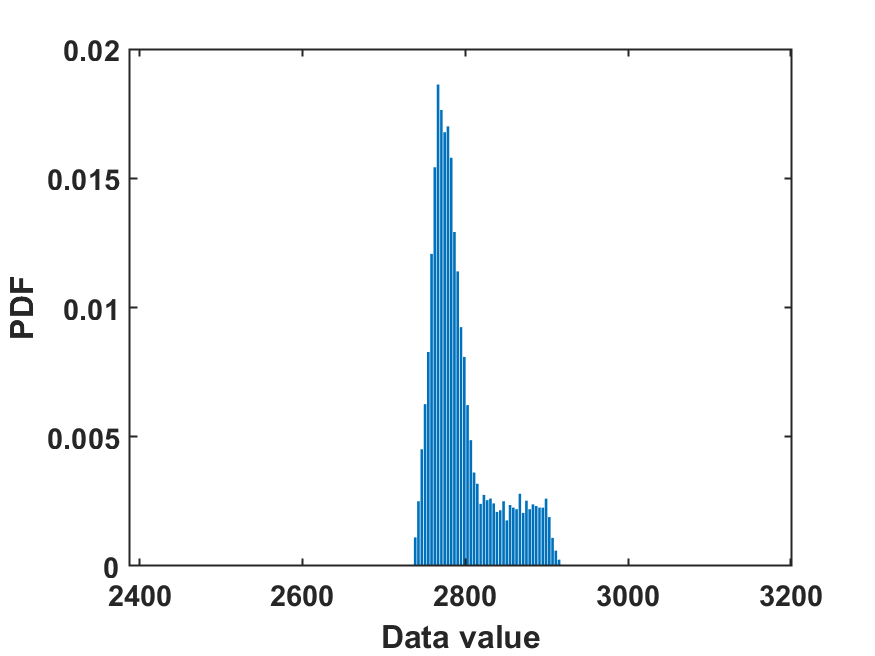
\includegraphics[width=0.35\columnwidth]{RDHentire.png} 
	\caption{Relative density histogram for entire dataset}
\end{figure}

The codes for ploting a relative density histogram
\begin{lstlisting}[language=Matlab,escapeinside=``]
x0=(nanmean(D)-nanstd(D)*10):nanstd(D)/10:(nanmean(D)+nanstd(D)*10);% give the central points
N=hist(D,x0); % get the number of ranges
RDH=N/sum(N*nanstd(D)/10); % relative density histogram
figure;clf
bar(x0,RDH) % plot the relative density histogram
xlabel('Data value')% for the label of x axis
ylabel('PDF')% for the label of y axis
set(gca,'LineWidth',1,'FontSize',14,'FontWeight','bold')

print('RDHentire','-dpng')
\end{lstlisting}


%----------------------------------------------------------------------------------------

\section*{Question 3}

\begin{problem}
 Randomly sample 10 measurements from the elevations.txt dataset. Calculate the minimum, maximum, and mean elevation.
\end{problem}

%------------------------------------------------

\subsection*{Answer} 

The codes for randomly sampling 10 measurements

\begin{lstlisting}[language=Matlab,escapeinside=``]
d2=randsample(D,10,true); % Randomly sample 10 measurements from the elevations
max_d2=nanmax(d2) %calculate the maximum and print it in command window
min_d2=nanmin(d2) %calculate the minimum and print it in command window
mean_d2=nanmean(d2) % calcualate the mean and print it in command window
\end{lstlisting}

The results I got are that maximum value equals to 2.9046e+03, minimum value equals to 2.7694e+03, mean value equals to 2.8269e+03 and the standard deviation is 52.7902.




%----------------------------------------------------------------------------------------

\section*{Question 4 }

\begin{problem}
Repeat 1000 times, storing the mean, standard deviation, minimum, and maximum elevation each time.
\end{problem}




%------------------------------------------------

\subsection*{Answer}

The codes for repeating 1000 times:
\begin{lstlisting}[language=Matlab,escapeinside=``]
nMC=1000; % times of repetition
nsamp=10; %Number of size
Dstats=zeros(nMC,4)*NaN;%Initializes the storage matrix

for m=1:nMC
d1=randsample(D,nsamp,true); % Randomly sample 10 measurements from the elevations
Dstats(m,:)=[nanmin(d1) nanmax(d1) nanmean(d1) nanstd(d1)] ;%storing the minimum, maximum,
%mean,and standard deviation of elevation each time.

end
\end{lstlisting}


%----------------------------------------------------------------------------------------

\section*{Question 5 }

\begin{problem}
Plot a relative density histogram of each statistic.

\end{problem}

%------------------------------------------------

\subsection*{Answer}

The result is

\begin{figure}[htbp]
	\centering
	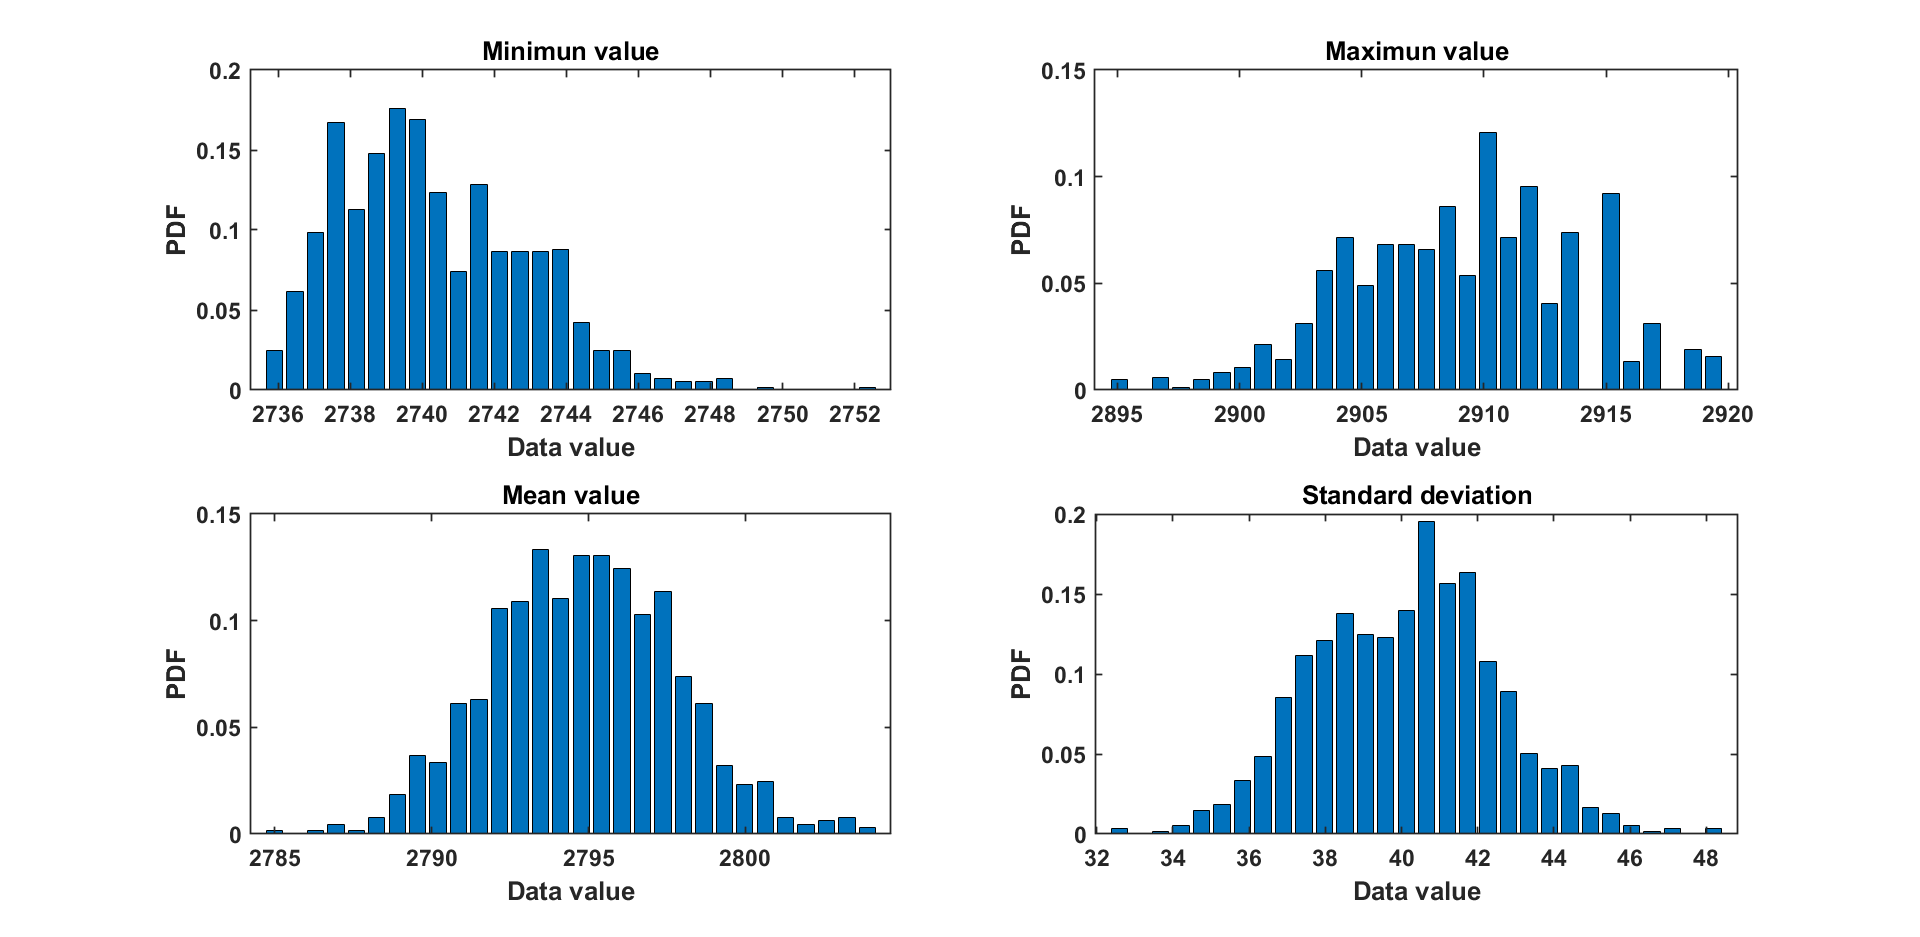
\includegraphics[width=0.9\columnwidth]{RDHsample.png} 
	\caption{Relative density histogram for samples' statistic}
\end{figure}

The codes for ploting relative density histograms of each statistic. I use a plotRDH function, the function can be seen in appendix

\begin{lstlisting}[language=Matlab,escapeinside=``]
bins=30;% bins for histogram
figure
subplot(2,2,1)
plotRDH(Dstats(:,1),bins);%relative density histogram for the minimun value
title('Minimun value')
subplot(2,2,2)
plotRDH(Dstats(:,2),bins);%relative density histogram for the maximun value
title('Maximun value')
subplot(2,2,3)
plotRDH(Dstats(:,3),bins);%relative density histogram for the mean value
title('Mean value')
subplot(2,2,4)
plotRDH(Dstats(:,4),bins);%relative density histogram for the standard deviation value
title('Standard deviation')
print('RDHsample','-dpng')
\end{lstlisting}



\section*{Question 6 }

\begin{problem}
The Gaussian (normal) distribution has the form
\begin{equation}
f\left( {x;\mu ,{\sigma ^2}} \right) = \frac{1}{{\sigma \sqrt {2\pi } }}{e^{ - \frac{{{{(x - \mu )}^2}}}{{2{\sigma ^2}}}}}
\end{equation}
for mean $\mu $ and standard deviation  $\sigma $.Fit the Gaussian distribution to
the entire elevation data set, using the true mean $\mu $ and true standard deviation $\sigma $.. Plot this
Gaussian curve on the same plot as your relative density histogram.
	
\end{problem}

\subsection*{Answer}

The result is

\begin{figure}[htbp]
	\centering
	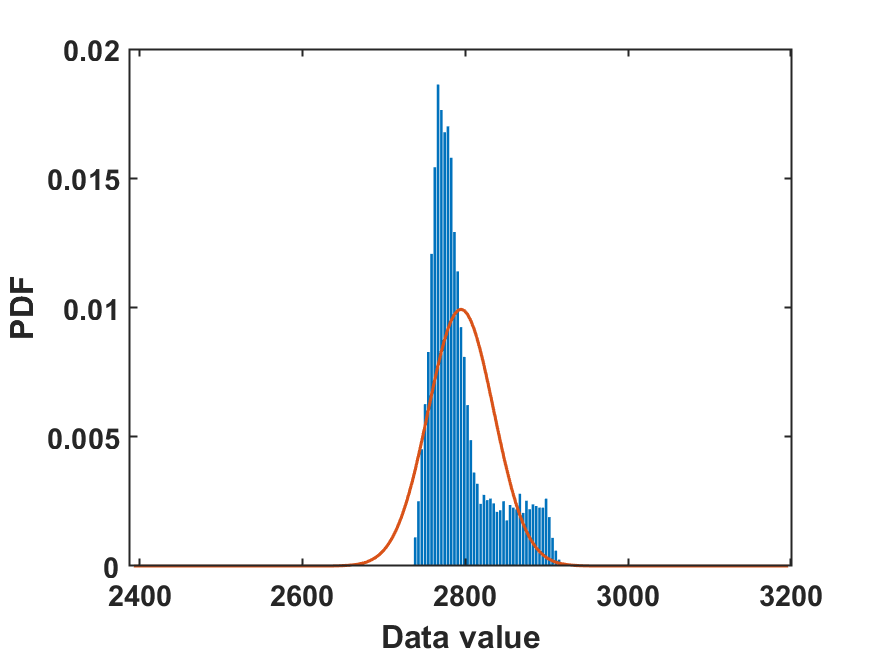
\includegraphics[width=0.7\columnwidth]{RDHGaussentire.png} 
	\caption{Relative density histogram for the entire dataset with Gaussian curve}
\end{figure}


The codes for plot Gaussian curve on the same plot as relative density histogram for the entire dataset

\begin{lstlisting}[language=Matlab,escapeinside=``]
x0=(nanmean(D)-nanstd(D)*10):nanstd(D)/10:(nanmean(D)+nanstd(D)*10);% give the central points
N=hist(D,x0); % get the number of ranges
RDH=N/sum(N*nanstd(D)/10); % relative density histogram
figure;clf
bar(x0,RDH) % plot the relative density histogram
hold on
plot(x0,mynormpdf(x0,mu,sigma),'LineWidth',1.5) % plot the Gaussian curve
xlabel('Data value')% for the label of x axis
ylabel('PDF')% for the label of y axis
set(gca,'LineWidth',1,'FontSize',14,'FontWeight','bold')
print('RDHGaussentire','-dpng')

\end{lstlisting} 


%----------------------------------------------------------------------------------------

\clearpage

\section*{Question 7 }

\begin{problem}
Fit the Gaussian distribution to each sample statistic, using your new dataset from the 1000
random subsample datasets of elevation - you have a dataset of 1000 values of $\hat{\mu}, \hat{\sigma}, \hat{q}_{0}, \hat{q}_{100} $.
Each of these sample statistics has a sample mean and sample standard deviation value that
can be used as the parameters in the Gaussian distribution formula. Plot the Gaussian curves
on your relative density histograms from above.
	
\end{problem}

The result is

\begin{figure}[htbp]
	\centering
	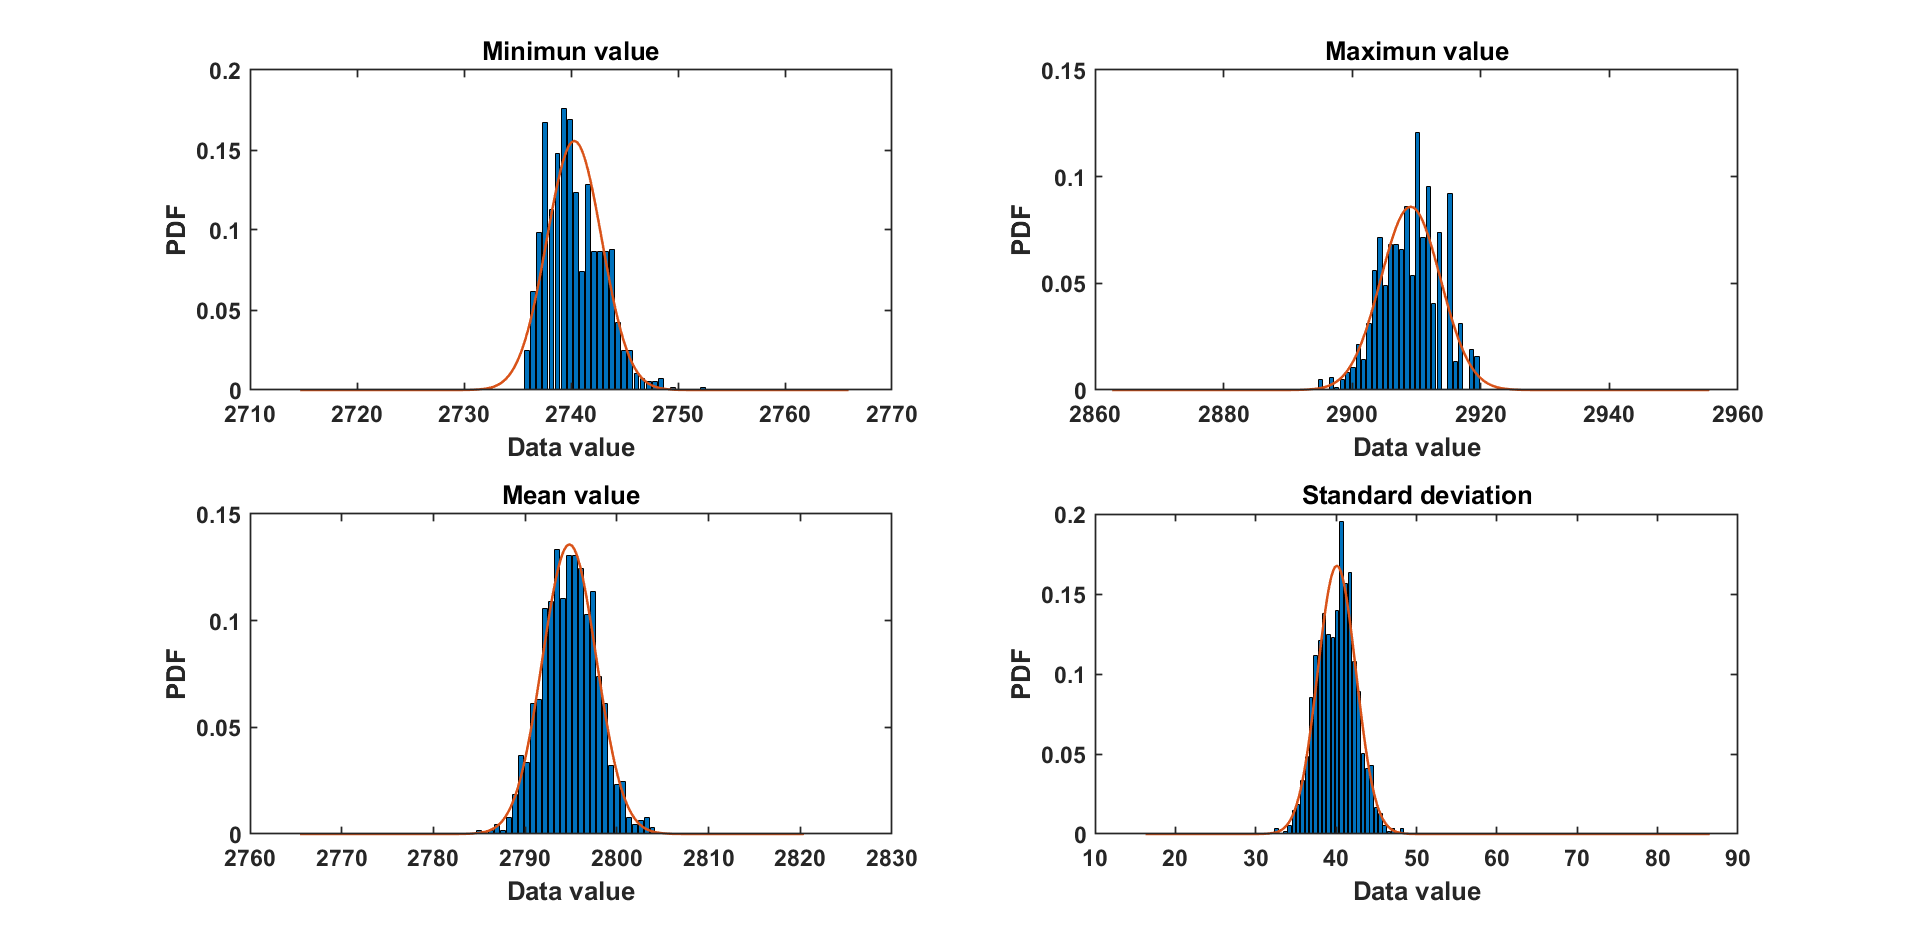
\includegraphics[width=1\columnwidth]{RDHGausssample.png} 
	\caption{Relative density histogram for each statistic with Gaussian curve}
\end{figure}

The codes for ploting the Gaussian curves
on  relative density histograms for four statistics

\begin{lstlisting}[language=Matlab,escapeinside=``]
x0_min=(mean(Dstats(:,1))-std(Dstats(:,1))*10):std(Dstats(:,1))/10:(mean(Dstats(:,1))+...
std(Dstats(:,1))*10); % set the points for Gaussian curve of minimum value of sample

x0_max=(mean(Dstats(:,2))-std(Dstats(:,2))*10):std(Dstats(:,2))/10:(mean(Dstats(:,2))+...
std(Dstats(:,2))*10); % set the points for Gaussian curve of maximum value of sample

x0_mean=(mean(Dstats(:,3))-std(Dstats(:,3))*10):std(Dstats(:,3))/10:(mean(Dstats(:,3))+...
std(Dstats(:,1))*10); % set the points for Gaussian curve of mean value of sample

x0_std=(mean(Dstats(:,4))-std(Dstats(:,4))*10):std(Dstats(:,4))/10:(mean(Dstats(:,4))+...
std(Dstats(:,2))*10); % set the points for Gaussian curve of standard deviation of sample


bins=30;% bins for histogram
figure
subplot(2,2,1)
plotRDH(Dstats(:,1),bins);%relative density histogram for the minimun value
hold on
plot(x0_min,mynormpdf(x0_min,mean(Dstats(:,1))...
,std(Dstats(:,1))),'LineWidth',1.5) % plot the Gaussian curve for minimum value
title('Minimun value')
subplot(2,2,2)
plotRDH(Dstats(:,2),bins)%relative density histogram for the maximun value
hold on
plot(x0_max,mynormpdf(x0_max,mean(Dstats(:,2))...
,std(Dstats(:,2))),'LineWidth',1.5) % plot the Gaussian curve for maximum value
title('Maximun value')
subplot(2,2,3)
plotRDH(Dstats(:,3),bins)%relative density histogram for the mean value
hold on
plot(x0_mean,mynormpdf(x0_mean,mean(Dstats(:,3))...
,std(Dstats(:,3))),'LineWidth',1.5) % plot the Gaussian curve for maximum value
title('Mean value')
subplot(2,2,4)
plotRDH(Dstats(:,4),bins)%relative density histogram for the standard deviation value
hold on
plot(x0_std,mynormpdf(x0_std,mean(Dstats(:,4))...
,std(Dstats(:,4))),'LineWidth',1.5) % plot the Gaussian curve for maximum value
title('Standard deviation')

print('RDHGausssample','-dpng')

\end{lstlisting}







\section*{Question 8 }

\begin{problem}
What is the probability of measuring a value less than the true mean?
\end{problem}


\subsection*{Answer}
The codes for get the probability of measuring a value less than the true mean

\begin{lstlisting}[language=Matlab,escapeinside=``]
Pro_less_mean=length(D(D<mu))/length(D)%get the probability of measuring a value less than the true mean
\end{lstlisting}

The result is  0.6590.


\clearpage
\section*{Question 9 }

\begin{problem}
What is the probability of measuring a minimum and maximum value within 1\% of the true value?
\end{problem}

\subsection*{Answer}

I got the result of probability of measuring a minimum  within 1\% of the true value is 0.8460 and the probability of that in maximum value is  0.3350. An interesting find is that these probability is same as the probability of less than 1\% of the true value in minimum value and larger than 1\% of the true value in maximum value. It is easy to understand, because the sample minimum value cannot smaller than the true minimum value and tha sample maximum value cannot larger than true maximum value.
 
 \begin{lstlisting}[language=Matlab,escapeinside=``]
samplemin=Dstats(:,1);% the minimum value 
samplemax=Dstats(:,2);% the minimum value 
indexmin1=find(samplemin<(q0*1.01)); %find the index for less than 1% of true min
indexmin2=find((samplemin>q0*0.99)&(samplemin<q0*1.01)); %find the index for within 1% of true min

Pmin_less01=length(indexmin1)/nMC%got the min<true min*1%
Pmin_within01=length(indexmin2)/nMC%got the min within true min*1%

indexmax1=find(samplemax>q100*0.99); %find the index for less than 1% of true max
indexmax2=find(samplemax>q100*0.99&samplemin<q100*1.01);%find the index for within 1% of true max
Pmax_less01=length(indexmax1)/nMC%got the min<true min*1%
Pmax_within01=length(indexmax2)/nMC%got the min within true min*1%
\end{lstlisting}
 

 
 \section*{Question 10 }
 
 \begin{problem}
 What is the range of elevations that contains 68\% of your measured mean values?
 	
 \end{problem}
 
 \subsection*{Answer}
 
I found a picture from wikipedia that said About 68\% of values drawn from a normal distribution are within one standard deviation $\sigma$ away from the mean. Therefore, I also use the range of  $\mu-\sigma,\mu-\sigma$ in measured mean values. The result shows that the probability is close to 68\%. The probability of between range $\mu-\sigma,\mu-\sigma$ is 0.6720, which is close to 68\%. The codes for calculating the probability are

\begin{figure}[htbp]
	\centering
	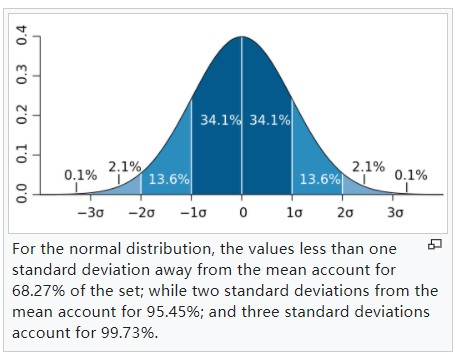
\includegraphics[width=0.8\columnwidth]{wiki.jpg} 
	\caption{picture from \url{https://en.wikipedia.org/wiki/Normal\_distribution}}
\end{figure}
 
\begin{lstlisting}[language=Matlab,escapeinside=``]
Dsamlemean=Dstats(:,3); %get the sample mean values
meansample_mean=mean(Dsamlemean); %get the mean of sample mean values
stdsample_mean=std(Dsamlemean);%get the standard deviataion of sample mean values

Pro_68=length(Dsamlemean((meansample_mean-stdsample_mean)...
<Dsamlemean&Dsamlemean<(meansample_mean+stdsample_mean)))/length(Dsamlemean)%use the range \mu-\sigma,\mu-\sigma to get probability
\end{lstlisting}
 
 

 \section*{Question 11 }

\begin{problem}
Vary your sample size and plot the sample statistics along with their uncertainties, as a
function of sample size.
	
\end{problem}

\subsection*{Answer}

The results are

\begin{figure}[htbp]
	\centering
	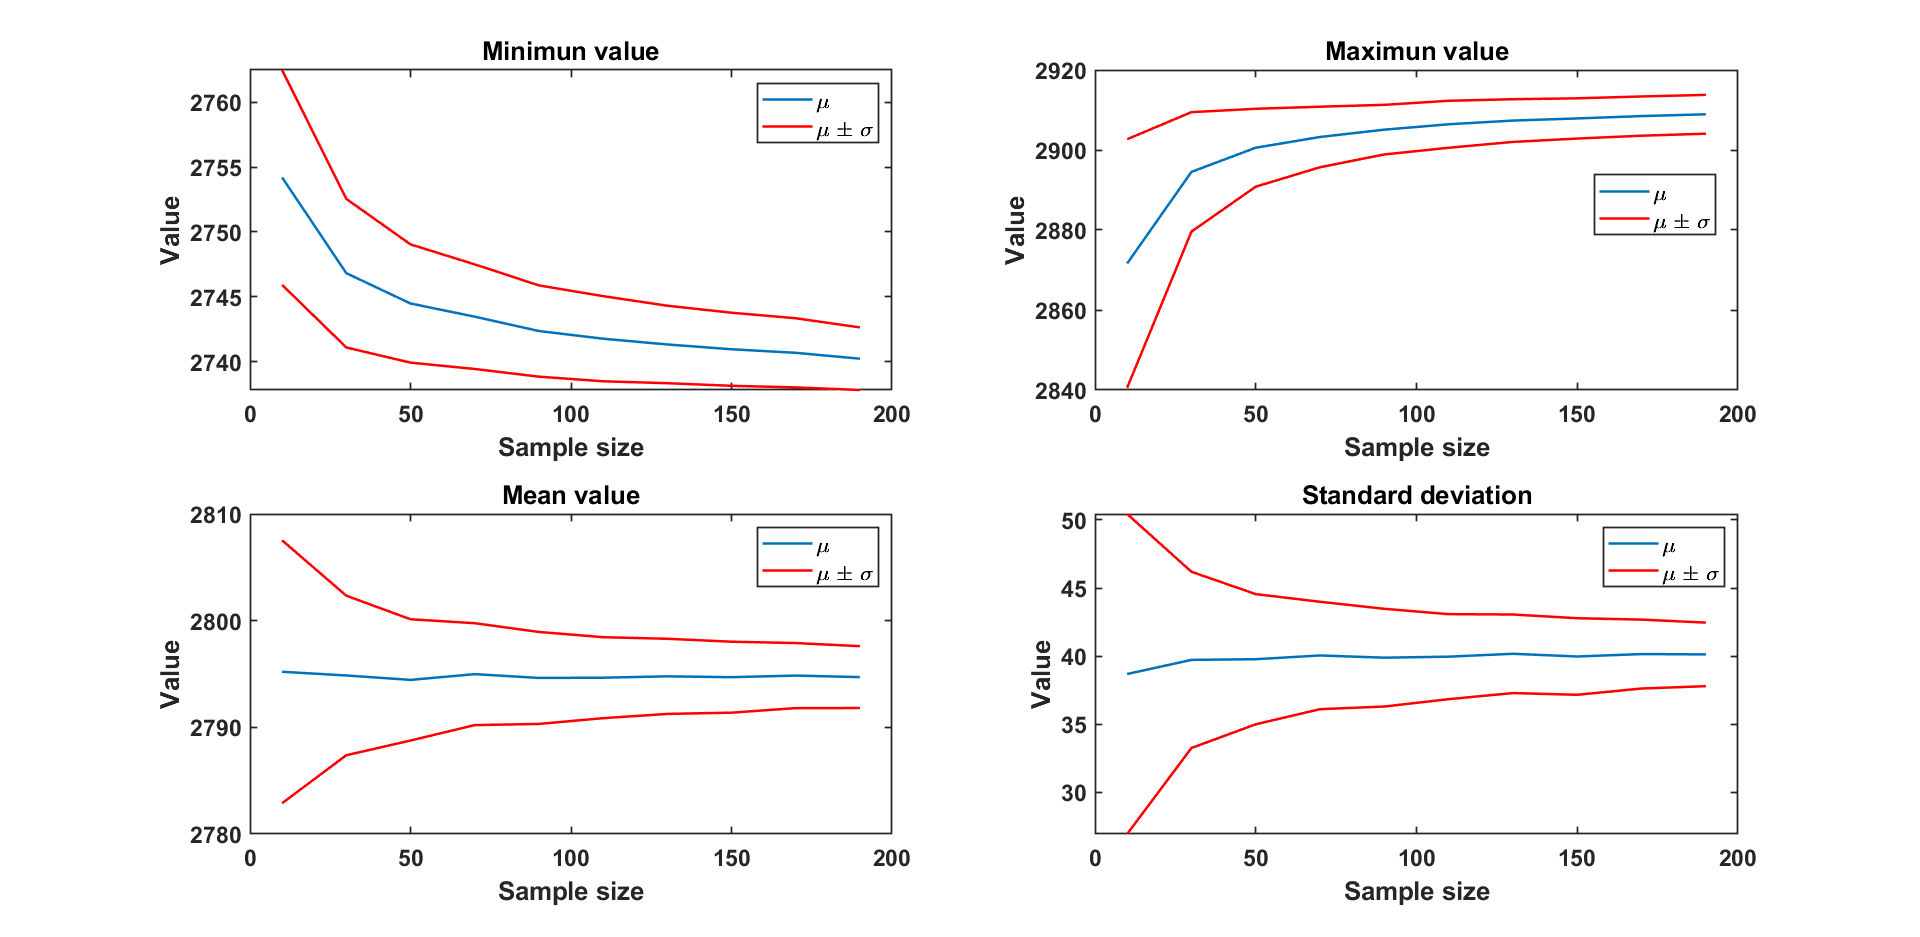
\includegraphics[width=0.8\columnwidth]{sampleuncern.png} 
	\caption{ The sample statistics along with their uncertainties with varying sample size}
\end{figure}

The codes for ploting the sample statistics along with their uncertainties with varying sample size


  \begin{lstlisting}[language=Matlab,escapeinside=``]
nMC=1000; % times of repetition
nsamp=[10:20:200]; %Number of size
Dstats=zeros(nMC,4)*NaN;%Initializes the storage matrix

for n=1:length(nsamp)
for m=1:nMC
d1=randsample(D,nsamp(n),true); % Randomly sample 10 measurements from the elevations
Dstats(m,:)=[nanmin(d1) nanmax(d1) nanmean(d1) nanstd(d1)] ;%storing the minimum, maximum,
%mean,and standard deviation of elevation each time.
end
sample_min_mean(n)=mean(Dstats(:,1));% get the mean of samle minimum value
sample_min_std(n)=std(Dstats(:,1));% get the standard deviation of samle minimum value

sample_max_mean(n)=mean(Dstats(:,2));% get the mean of samle maximum value
sample_max_std(n)=std(Dstats(:,2));% get the standard deviation of samle maximum value

sample_mean_mean(n)=mean(Dstats(:,3));% get the mean of samle mean value
sample_mean_std(n)=std(Dstats(:,3)); % get the standard deviation of samle mean value   

sample_std_mean(n)=mean(Dstats(:,4));% get the mean of samle standard deviation value
sample_std_std(n)=std(Dstats(:,4));  % get the standard deviation of samle standard deviation value
end
figure

subplot(2,2,1)
plot(nsamp,sample_min_mean,'LineWidth',1.5);%plot the mean of samle minimum value
hold on
plot(nsamp,sample_min_mean+sample_min_std,nsamp,sample_min_mean-sample_min_std...
,'LineWidth',1.5,'color','r');%plot the uncertainties of the mean of samle minimum value
title('Minimun value')
legend('\mu','\mu \pm \sigma') %give the legend
set(gca,'LineWidth',1,'FontSize',14,'FontWeight','bold')
subplot(2,2,2)
plot(nsamp,sample_max_mean,'LineWidth',1.5);%plot the mean of samle maximum value
hold on
plot(nsamp,sample_max_mean+sample_max_std,nsamp,sample_max_mean-sample_max_std...
,'LineWidth',1.5,'color','r');%plot the uncertainties of the mean of samle maximum value
title('Maximun value')
legend('\mu','\mu \pm \sigma') %give the legend
set(gca,'LineWidth',1,'FontSize',14,'FontWeight','bold')
subplot(2,2,3)
plot(nsamp,sample_mean_mean,'LineWidth',1.5);%plot the mean of samle mean value
hold on
plot(nsamp,sample_mean_mean+sample_mean_std,nsamp,sample_mean_mean-sample_mean_std...
,'LineWidth',1.5,'color','r');%plot the uncertainties of the mean of samle mean value
title('Mean value')
legend('\mu','\mu \pm \sigma') %give the legend
set(gca,'LineWidth',1,'FontSize',14,'FontWeight','bold')
subplot(2,2,4)
plot(nsamp,sample_std_mean,'LineWidth',1.5);%plot the mean of samle standard deviation value
hold on
plot(nsamp,sample_std_mean+sample_std_std,nsamp,sample_std_mean-sample_std_std...
,'LineWidth',1.5,'color','r');%plot the uncertainties of the mean of samle standard deviation value
title('Standard deviation')
legend('\mu','\mu \pm \sigma') %give the legend
set(gca,'LineWidth',1,'FontSize',14,'FontWeight','bold')
print('sampleuncern','-dpng')

\end{lstlisting}

 \section*{Question 12 }

\begin{problem}
Plot the relative density histogram and normal pdf for uniform sampling with a spacing of 200
meters. Assume the dataset spans 1000m x 1000m, and sample uniformly in both directions.
	
\end{problem}

\subsection*{Answer}

The result is

\begin{figure}[htbp]
	\centering
	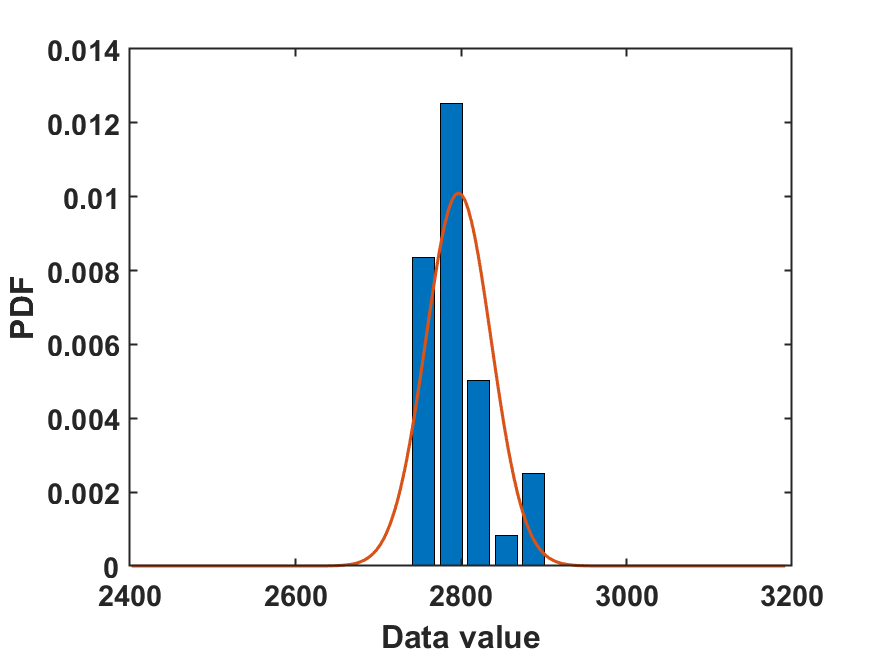
\includegraphics[width=0.8\columnwidth]{samplespace1.png} 
	\caption{ the relative density histogram and normal pdf for uniform sampling with a spacing of 200}
\end{figure}

The codes for ploting the relative density histogram and normal pdf for uniform sampling with a spacing of 200
meters.

\begin{lstlisting}[language=Matlab,escapeinside=``]
D=load('elevations.txt');%load the data again
space=200; % define the space
dx=space/10;% the interval of x axis
dy=space/10;% the interval of y axis
[nr,nc]=size(D); %get the size of dataset


mm=1;%initialize the matrix index
for ix=1:dx:nr
for iy=1:dy:nc
unisample(mm)=D(ix,iy);%store the sample
mm=mm+1;%index for stroring the next sample     
end
end

x0_sample=(nanmean(unisample)-nanstd(unisample)*10):nanstd(unisample)/10:(nanmean(unisample)+...
nanstd(unisample)*10); % set the points for Gaussian curve of standard deviation of sample
figure
bins=5;% give the bin numbers
plotRDH(unisample,bins);%relative density histogram for the standard deviation value
hold on
plot(x0_sample,mynormpdf(x0_sample,nanmean(unisample)...
,nanstd(unisample)),'LineWidth',1.5) % plot the Gaussian curve for samples
print('samplespace1','-dpng')
\end{lstlisting}

\clearpage
 \section*{Question 13 }

\begin{problem}
Repeat for uniform sampling with a spacing of 30 meters.
	
\end{problem}

\subsection*{Answer}
The result is

\begin{figure}[htbp]
	\centering
	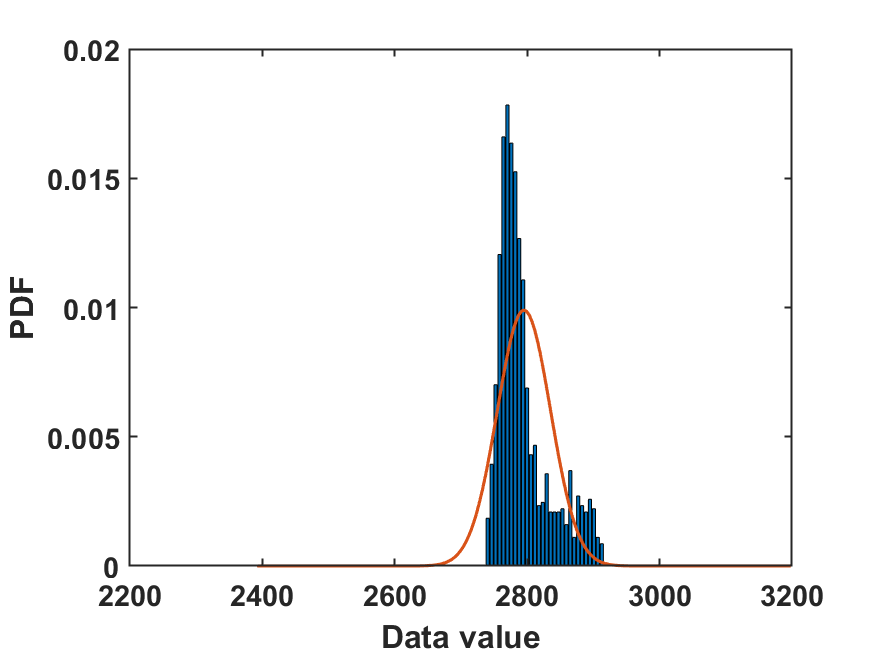
\includegraphics[width=0.8\columnwidth]{samplespace2.png} 
	\caption{ the relative density histogram and normal pdf for uniform sampling with a spacing of 30}
\end{figure}

The codes for uniform sampling with a spacing of 30 meters

\begin{lstlisting}[language=Matlab,escapeinside=``]
space=30; % define the space
dx=space/10;% the interval of x axis
dy=space/10;% the interval of y axis
[nr,nc]=size(D); %get the size of dataset



mm=1;%initialize the matrix index
for ix=1:dx:nr
for iy=1:dy:nc
unisample(mm)=D(ix,iy);%store the sample
mm=mm+1;%index for stroring the next sample     
end
end

figure
x0_sample=(nanmean(unisample)-nanstd(unisample)*10):nanstd(unisample)/10:(nanmean(unisample)+...
nanstd(unisample)*10); % set the points for Gaussian curve of standard deviation of sample

bins=30;% give the bin numbers
plotRDH(unisample,bins);%relative density histogram for the standard deviation value
hold on
plot(x0_sample,mynormpdf(x0_sample,nanmean(unisample)...
,nanstd(unisample)),'LineWidth',1.5) % plot the Gaussian curve for samples
print('samplespace2','-dpng')
\end{lstlisting}

\section*{Question 14 }

\begin{problem}
Plot the sample statistics and their uncertainties for uniform sampling, as a function of sample
size.
	
\end{problem}

\subsection*{Answer}
I plot both sample statistics towards space and sample size.  The result are

\begin{figure}[htbp]
	\centering
	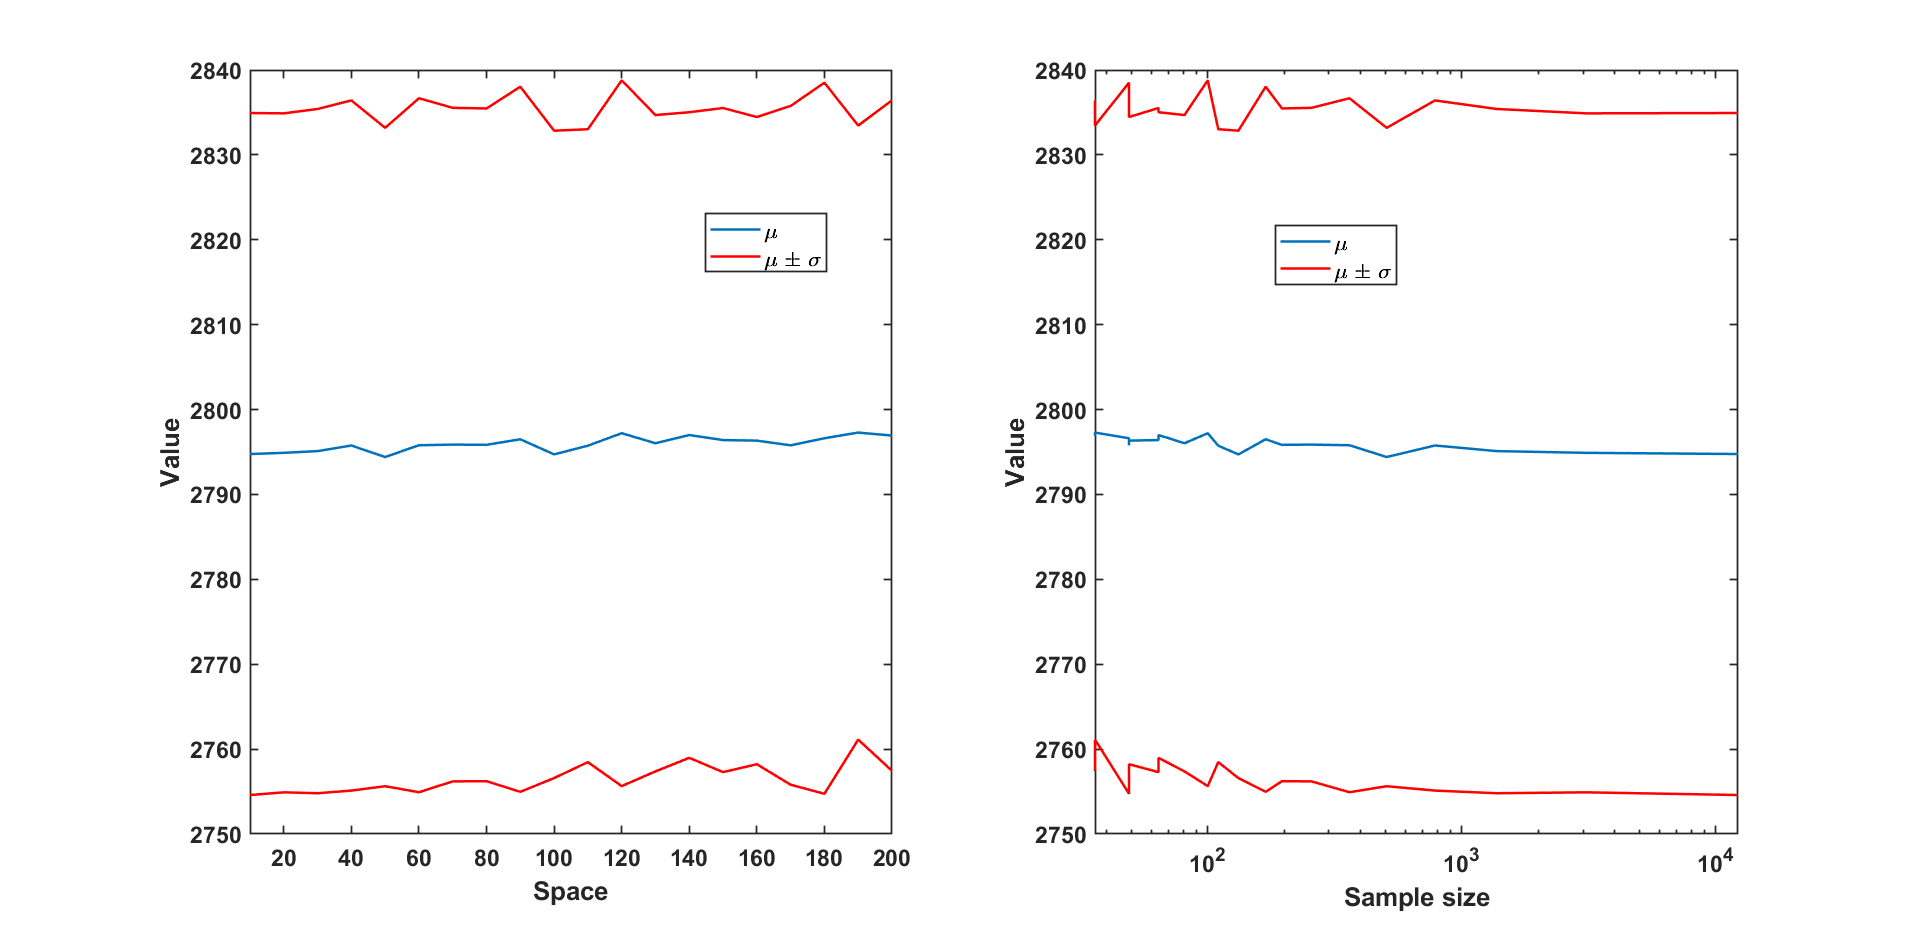
\includegraphics[width=0.8\columnwidth]{samplespace3.png} 
	\caption{ Sample statistics and their uncertainties for uniform sampling with different sample size}
\end{figure}

The codes for ploting the sample statistics and their uncertainties for uniform sampling, as a function of sample
size.
\begin{lstlisting}[language=Matlab,escapeinside=``]

space=[10:10:200]; % define the space

[nr,nc]=size(D); %get the size of dataset

Dstore=zeros(length(space),2)*NaN; %Initializes the storage matrix

for ii=1:length(space)
dx=space(ii)/10;% the interval of x axis
dy=space(ii)/10;% the interval of y axis
mm=1;%initialize the matrix index
unisample=[];
for ix=1:dx:nr
for iy=1:dy:nc
unisample(mm)=D(ix,iy);%store the sample
mm=mm+1;%index for stroring the next sample
end
end
len(ii)=length(unisample);
Dstore(ii,1:2)=[nanmean(unisample) nanstd(unisample)];%storing the minimum, maximum,
%mean,and standard deviation of elevation each time.
end

figure
subplot(1,2,1)
plot(space,Dstore(:,1),'LineWidth',1.5);%plot the mean value
hold on
plot(space,Dstore(:,1)+Dstore(:,2),space,Dstore(:,1)-Dstore(:,2)...
,'LineWidth',1.5,'color','r');%plot the uncertainties of the mean value
legend('\mu','\mu \pm \sigma') %give the legend
xlabel('Space')
ylabel('Value')
xlim([10,200])
set(gca,'LineWidth',1,'FontSize',14,'FontWeight','bold')

subplot(1,2,2)
semilogx(len,Dstore(:,1),'LineWidth',1.5);%plot the mean value
hold on
semilogx(len,Dstore(:,1)+Dstore(:,2),len,Dstore(:,1)-Dstore(:,2)...
,'LineWidth',1.5,'color','r');%plot the uncertainties of the mean value
legend('\mu','\mu \pm \sigma') %give the legend
xlabel('Sample size')
ylabel('Value')
xlim([36,max(len)])
set(gca,'LineWidth',1,'FontSize',14,'FontWeight','bold')
print('samplespace3','-dpng')
\end{lstlisting}

\appendix{Appendix}

Codes in plotPRH.m
\begin{lstlisting}[language=Matlab,escapeinside=``]
space=[10:10:200]; % define the space
dx=space/10;% the interval of x axis
dy=space/10;% the interval of y axis
[nr,nc]=size(D); %get the size of dataset

Dstore=zeros(length(space),2)*NaN; %Initializes the storage matrix

for ii=1:length(space)

mm=1;%initialize the matrix index
for ix=1:dx:nr
for iy=1:dy:nc
unisample(mm)=D(ix,iy);%store the sample
mm=mm+1;%index for stroring the next sample
end
end
Dstore(ii,1:2)=[nanmean(unisample) nanstd(unisample)];%storing the minimum, maximum,
%mean,and standard deviation of elevation each time.
end

figure

plot(space,Dstore(:,1),'LineWidth',1.5);%plot the mean value
hold on
plot(space,Dstore(:,1)+Dstore(:,2),space,Dstore(:,1)-Dstore(:,2)...
,'LineWidth',1.5,'color','r');%plot the uncertainties of the mean value
legend('\mu','\mu \pm \sigma') %give the legend
xlabel('Space')
ylabel('Value')
xlim([10,200])
set(gca,'LineWidth',1,'FontSize',14,'FontWeight','bold')
print('samplespace3','-dpng')
\end{lstlisting}
\end{document}
